\documentclass[]{scrreprt}
\usepackage{amsmath,amsfonts,graphicx}
%\usepackage{multirow}
%\usepackage{pslatex}
%\usepackage{tabularx}
%\usepackage{comment}
%\usepackage{xspace}
%\usepackage{array}

%\usepackage{hyperref}

%\usepackage{caption}
%\DeclareCaptionFont{white}{\color{white}}
%\DeclareCaptionFormat{listing}{\colorbox{gray}{\parbox{\textwidth}{#1#2#3}}}

\def\species{\mathrm{sp}}
\def\phase{\mathrm{ph}}
\def\massfrac{\chi}
\def\flux{\mathbf{F}}
\def\darcyvel{\mathbf{v}}
\def\energydens{\mathcal{E}}
\def\d{\mathrm{d}}

\newcommand{\uo}{\mbox{UO\textsubscript{2}}\xspace}

\setcounter{secnumdepth}{3}


\begin{document}


\title{Sinks Tests}
\author{CSIRO}
\maketitle

\tableofcontents

\chapter{PorousFlow sink boundary conditions}

A number of different sink boundary conditions have been implemented
in PorousFlow.  (To make these into sources instead of sinks, the
strength of the flux just needs to be made negative.)  All the sinks
are implemented using full upwinding.  This is to prevent the sink
from attempting to remove fluid from a node that actually contains no
fluid.

The basic sink uses a Function to specify the flux on the boundary,
and also has the option of multiplying by any combination of: the
fluid mobility, the relative permeability, or a mass fraction.  These
latter multiplying factors are all useful in the case of sinks to
prevent an unlimited amount of fluid being withdrawn from the porous
medium, which can lead to extremely poor nonlinear convergence even if
only one node in the entire mesh is ``running dry''.

Derived from the basic one, is another boundary condition that allows
the flux to be modified by a piecewise-linear function of
porepressure, which is useful for the case where transfer coefficients
are defined across the boundary, or more complicated situations.

Also derived from the basic one are two others, in which the flux is
governed by a half Gaussian or half cubic function of porepressure,
which are useful for modelling evapotranspiration through a boundary.

\section{Basic sink}
\label{basic.sec}

\subsection{Test 1}

A sink flux of strength 6\,kg.m$^{-2}$.s$^{-1}$ is applied to the left
edge ($x=0$) of a 3D mesh.  A single-phase, single-component fluid is
used, and the porepressure is initialised to $p=y+1$ (for $0\leq y\leq
1$).  No fluid flow within the element is used, so the masses of fluid
at the finite-element nodes behave independently.  The fluid is
assumed to have density $\rho = 1.1 \exp(p/1.3)$ [kg.m$^{-3}$].  The
porosity is 0.1.

Under these conditions, assuming $p\geq 0$ so that the porous medium
is fully saturated with fluid, the fluid mass at a node should obey
\begin{equation}
m = V\phi\rho = V\times0.1\times 1.1\exp(p/1.3) = m(t=0) - 6At \ ,
\end{equation}
where $V$ is the volume occupied by the node, and $A$ is its area
exposed to the flux.  MOOSE correctly produces this result, as
illustrated in Figure~\ref{s01.fig}.

\begin{figure}[htb]
\begin{center}
\includegraphics[width=8cm]{s01.pdf}
\caption{Results of Test 1, illustrating that MOOSE correctly applies
  a constant sink flux to boundary nodes.}
\label{s01.fig}
\end{center}
\end{figure}

\subsection{Test 2}

An identical setup to Test 1 is used here, but with the sink flux
strength being multiplied by the mobility:
\begin{equation}
\mbox{mobility} = n_{i}k_{ij}n_{j}\rho/\nu \ ,
\end{equation}
where $n_{i}k_{ij}n_{j}$ is the permeability tensor $k$ projected onto
the normal direction to the boundary $n$, and the fluid density and
viscosity are $\rho$ and $\nu$, respectively.  In this example
$\nu=1.1$\,Pa.s and $n_{i}k_{ij}n_{j}=0.2$\,m$^{2}$.  The other
parameters are the same as Test 1, except now the strength of the flux
is 6\,Pa.s$^{-1}$.

In this case, the expected result is (for $p>0$)
\begin{equation}
\frac{\d m}{\d t} = V\phi \frac{\d \rho}{\d t} = -6 A
\frac{n_{i}k_{ij}n_{j}\rho}{\mu} \ .
\end{equation}
MOOSE correctly produces this result, as illustrated in
Figure~\ref{s02.fig}.

\begin{figure}[htb]
\begin{center}
\includegraphics[width=8cm]{s02.pdf}
\caption{Results of Test 2, illustrating that MOOSE correctly applies
  a constant sink flux modified by the fluid mobility.  (A slight
  drift away from the expected result is due to MOOSE taking large
  time steps.)}
\label{s02.fig}
\end{center}
\end{figure}


\subsection{Test 3}

An identical setup to Test 1 is used here, but with the sink flux
strength being multiplied by the relative permeability, which is
chosen to be:
\begin{equation}
\kappa_{\mathrm{rel}} = S^{2} \ ,
\end{equation}
with $S$ being the fluid saturation.  A van-Genuchten capillary
relationship is used:
\begin{equation}
S = \left( 1 + (-\alpha p)^{1/(1-m)} \right)^{-m} \ ,
\end{equation}
with $\alpha = 1.1$\,Pa$^{-1}$, and $m=0.5$.  The porepressure is
initialised to be $p=-y$.  The other parameters are
identical to Test 1.

In this case, the expected result is
\begin{equation}
\frac{\d m}{\d t} = V\phi \frac{\d \rho S}{\d t} = -6 A S^{2} \ .
\end{equation}
MOOSE correctly produces this result, as illustrated in
Figure~\ref{s03.fig}.

\begin{figure}[htb]
\begin{center}
\includegraphics[width=8cm]{s03.pdf}
\caption{Results of Test 3, illustrating that MOOSE correctly applies
  a constant sink flux modified by the fluid relative permeability.}
\label{s03.fig}
\end{center}
\end{figure}


\subsection{Test 4}

A similar setup to Test 1 is used here, but with a 3-component,
single-phase fluid, with the sink flux only extracting the second
component, with a rate proportional to the mass fraction of that
component.  This test checks that the flux is correctly implemented
(see Figure~\ref{s07.fig}) and that the correct fluid component is being
withdrawn from the correct nodes.  MOOSE produces the expected result.

\begin{figure}[htb]
\begin{center}
\includegraphics[width=8cm]{s07.pdf}
\caption{Results of Test 4, illustrating that MOOSE correctly applies
  a sink flux of a particular fluid component proportional to the
  component's mass fraction.}
\label{s07.fig}
\end{center}
\end{figure}


\subsection{Test 5}

A sink is applied to the left edge ($x=0$) of a 3D mesh.  A
3-component, 2-phase fluid is used.  Call the two phases ``water'' and
``gas''.  The porepressures are initialised to $p_{\mathrm{water}} =
y$ and $p_{\mathrm{gas}} = y + 3$.  The mass fractions are initialised
to $(0.3, 0.35, 0.35)$ in the water phase, and $(0.1, 0.8, 0.1)$ in
the gas phase.  The water phase is assumed to have density
$\rho_{\mathrm{water}} = 1.5 \exp(p_{\mathrm{water}}/2.3)$, and the gas phase
$\rho_{\mathrm{gas}} = 1.1 \exp(p_{\mathrm{gas}}/1.3)$.  A van-Genuchten capillary
relationship is used:
\begin{equation}
S_{\mathrm{water}} = \left( 1 + (\alpha (p_{\mathrm{gas}} - p_{\mathrm{water}})^{1/(1-m)} \right)^{-m} \ ,
\end{equation}
with $\alpha = 1.1$\,Pa$^{-1}$, and $m=0.5$.  The water relative
permeaility is assumed to be Corey type with exponent $1$, and the gas
phase has exponent $2$ (that is $\kappa_{\mathrm{rel,gas}} =
S_{\mathrm{gas}}^{2}$, with $S_{\mathrm{gas}} = 1 -
S_{\mathrm{water}}$).

The sink flux acts only on the second component.  It is multiplied by the
relative permeability of the gas phase, and the mass fraction of the
second component in the gas phase.  This is possibly meaningless
physically, but acts as a good test of the PorousFlowSink.  In this
test the mass fractions remain fixed: there is nothing to induce a
change of a component from the water phase to the gas phase since the
only Kernels used are mass-conservation Kernels that simply demand
mass conservation of each fluid component (summed over each phase).

The test checks whether MOOSE is correctly applying the sink flux, and
that the fluid-component masses at the nodes respond correctly to the
flux.  Figure~\ref{s08.fig} demonstrates that MOOSE produces the
expected result.

\begin{figure}[htb]
\begin{center}
\includegraphics[width=8cm]{s08.pdf}
\caption{Results of Test 5, illustrating that in a 2-phase system
  MOOSE correctly applies a sink flux of a particular fluid component
  proportional to the component's mass fraction and the relative
  permeaility of the gas phase.}
\label{s08.fig}
\end{center}
\end{figure}



\section{Piecewise-linear sink}
\label{piecewise.sec}

A sink flux of strength
\begin{equation}
f = \left\{
\begin{array}{ll}
8 & \mbox{ if } p > 0.8 \\
8(p + 0.2) & \mbox{ if } 0.3 \leq p \leq 0.8 \\
4 & \mbox{ if } p < 0.3 \ ,
\end{array}
\right.
\end{equation}
(measured in kg.m$^{-2}$.s$^{-1}$) is applied to the right side
($x=1$) of a 3D mesh.  A single-phase, single-component fluid is used,
and the porepressure is initialised to $p=y+1$ (for $0\leq y \leq 1$).
No fluid flow within the element is used, so the masses of fluid at
the finite-element nodes behave independently.  The fluid is assumed
to have density $\rho = 1.1 \exp(p/1.3)$ [kg.m$^{-3}$].  The porosity
is 0.1.

Under these conditions, the expected result for the fluid mass at a
node on the right side of the mesh is
\begin{equation}
\frac{\d m}{\d t} = V\phi \frac{\d \rho S}{\d t} = -f A \ .
\end{equation}
The notation is the same as in previous sections.

The test checks that the mass evolves according to this equation, and
that the flux is applied correctly.  Figure~\ref{s04.fig} demonstrates
agreement with the expected flux and the MOOSE implementation.

\begin{figure}[htb]
\begin{center}
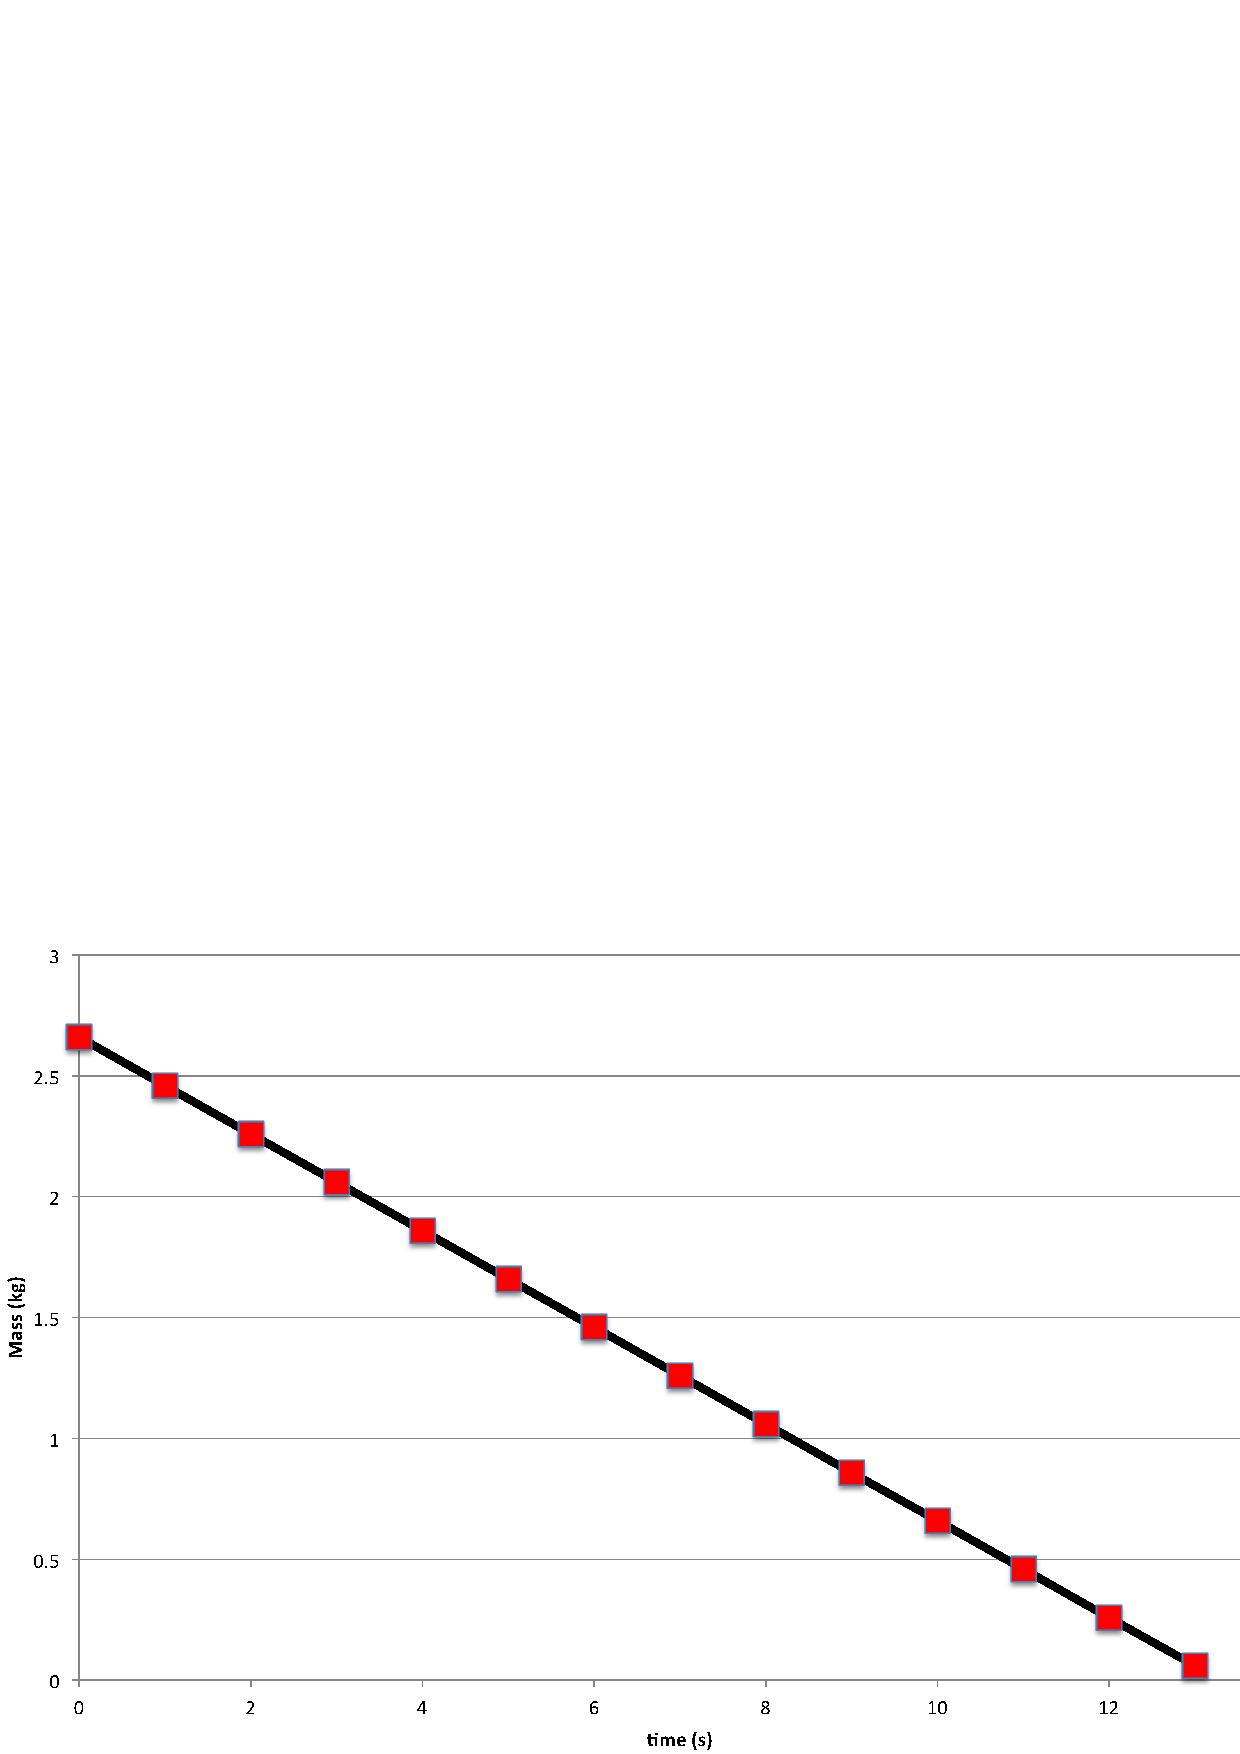
\includegraphics[width=8cm]{s04.pdf}
\caption{A piecewise-linear sink flux is correctly modelled by MOOSE}
\label{s04.fig}
\end{center}
\end{figure}



\section{Half-Gaussian sink}
\label{half_gaussian.sec}

A sink flux of strength
\begin{equation}
f = \left\{
\begin{array}{ll}
6 & \mbox{ if } p \geq 0.9 \\
6\exp\left(-\frac{1}{2} \left(\frac{p-0.9}{0.5} \right)^{2}\right) & \mbox { if } p < 0.9 \ .
\end{array}
\right.
\end{equation}
(measured in kg.m$^{-2}$.s$^{-1}$) is applied to the right side
($x=1$) of a 3D mesh.  This is a half-Gaussian sink with center
0.9\,Pa, standard deviation 0.5\,Pa and maximum 6.  A single-phase,
single-component fluid is used, and the porepressure is initialised to
$p=y+1.4$ (for $0\leq y \leq 1$).  No fluid flow within the element is
used, so the masses of fluid at the finite-element nodes behave
independently.  The fluid is assumed to have density $\rho = 1.1
\exp(p/1.3)$ [kg.m$^{-3}$].  The porosity is 0.1.  A van-Genuchten capillary
relationship is used:
\begin{equation}
S = \left( 1 + (-\alpha p)^{1/(1-m)} \right)^{-m} \ ,
\end{equation}
with $\alpha = 1.1$\,Pa$^{-1}$, and $m=0.5$.

Under these conditions, the expected result for the fluid mass at a
node on the right side of the mesh is
\begin{equation}
\frac{\d m}{\d t} = V\phi \frac{\d \rho S}{\d t} = -f A \ .
\end{equation}
The notation is the same as in previous sections.

The test checks that the mass evolves according to this equation, and
that the flux is applied correctly.  Figure~\ref{s05.fig} demonstrates
agreement with the expected flux and the MOOSE implementation.

\begin{figure}[htb]
\begin{center}
\includegraphics[width=8cm]{s05.pdf}
\caption{A half-Gaussian sink flux with center 0.9\,Pa and standard
  deviation 0.5\,Pa is correctly modelled by MOOSE}
\label{s05.fig}
\end{center}
\end{figure}



\section{Half-cubic sink}
\label{half_cubic.sec}

A sink flux of strength
\begin{equation}
f = \left\{
\begin{array}{ll}
3 & \mbox{ if } p \geq 0.9 \\
\frac{3}{(-0.8)^3} (2(p-0.9) + 0.8) (p - 0.9 + 0.8)^2 & \mbox{ if }
0.1 < p < 0.9 \\
0 & \mbox{ if } p \leq 0.1
\end{array}
\right.
\end{equation}
(measured in kg.m$^{-2}$.s$^{-1}$) is applied to the right side
($x=1$) of a 3D mesh.  This is a half-cubic sink with center
0.9\,Pa, cutoff $-0.8$\,Pa, and maximum 3\,kg.m$^{-2}$.s$^{-1}$.  A
single-phase, single-component fluid is used, and the porepressure is
initialised to $p=x(y+1)$ (for $0\leq y \leq 1$ and $0\leq x \leq 1$).
No fluid flow within the element is used, so the masses of fluid at
the finite-element nodes behave independently.  The fluid is assumed
to have density $\rho = 1.1 \exp(p/1.3)$ [kg.m$^{-3}$].  The porosity
is 0.1.

Under these conditions, the expected result for the fluid mass at a
node on the right side of the mesh is
\begin{equation}
\frac{\d m}{\d t} = V\phi \frac{\d \rho S}{\d t} = -f A \ .
\end{equation}
The notation is the same as in previous sections.

The test checks that the mass evolves according to this equation, and
that the flux is applied correctly.  Figure~\ref{s06.fig} demonstrates
agreement with the expected flux and the MOOSE implementation.

\begin{figure}[htb]
\begin{center}
\includegraphics[width=8cm]{s06.pdf}
\caption{A half-cubic sink with center 0.9\,Pa, cutoff $-0.8$\,Pa, and
  maximum 3\,kg.m$^{-2}$.s$^{-1}$ is correctly modelled by MOOSE.}
\label{s06.fig}
\end{center}
\end{figure}








\end{document}

